% SC1007 — Chapter 2: Stacks, Queues & Deques
% No \documentclass — included by modules/SC1007/main.tex (book class).
\chapter{Stacks, Queues \& Deques}
\label{ch:stacks-queues}

\begin{quote}
\emph{``Push, pop, enqueue, dequeue.''} --- Four operations, yet they power recursion, BFS, undo, and scheduling.
\end{quote}

\noindent\textbf{Prerequisites:} Ch.~1 (arrays/lists, $O(\cdot)$). This chapter adds restricted-access structures and classic applications.

\section*{Learning Outcomes}
After this chapter you will be able to:
\begin{enumerate}[label=(L\arabic*)]
    \item implement stacks/queues/deques via arrays and linked lists in $O(1)$;
    \item use stacks for matching, postfix evaluation, and recursion simulation;
    \item use queues for BFS preview and scheduling; explain circular buffers;
    \item choose among stack / queue / deque and analyse amortised costs.
\end{enumerate}

% ============================================================
\section{Stacks: LIFO}
\label{sec:stacks}
A \emph{stack} is LIFO: \texttt{push} adds at the top, \texttt{pop} removes from the top, \texttt{peek} inspects. All $\Theta(1)$.

\begin{figure}[h]
\centering
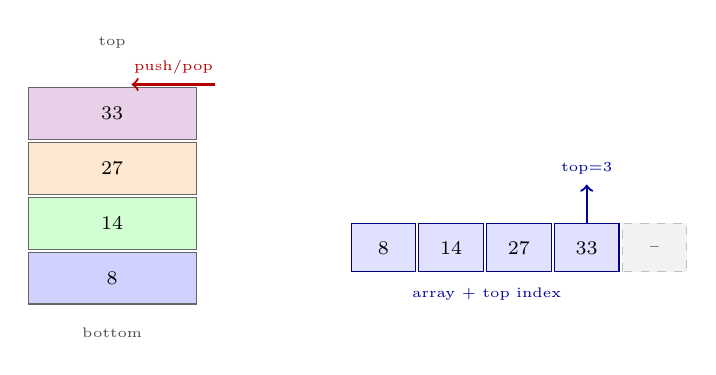
\begin{tikzpicture}[scale=0.82, every node/.style={font=\scriptsize}]
  \foreach \i/\c/\t in {0/blue!18/8,1/green!18/14,2/orange!18/27,3/violet!18/33} {
    \draw[fill=\c, draw=black!60] (0,\i*0.85) rectangle ++(2.6,0.8);
    \node at (1.3,\i*0.85+0.4) {\t};
  }
  \draw[->, thick, red!70!black] (2.9,3.4) -- (1.6,3.4) node[midway, above, font=\tiny] {push/pop};
  \node[font=\tiny, gray!60!black] at (1.3,-0.45) {bottom};
  \node[font=\tiny, gray!60!black] at (1.3,4.05) {top};
  \begin{scope}[xshift=5cm, yshift=0.5cm]
    \foreach \i/\v in {0/8,1/14,2/27,3/33} {
      \draw[fill=blue!12, draw=blue!50!black] (\i*1.05,0) rectangle ++(1.0,0.75);
      \node at (\i*1.05+0.5,0.37) {\v};
    }
    \draw[fill=gray!10, draw=gray!50, dashed] (4*1.05,0) rectangle ++(1.0,0.75);
    \node[font=\tiny] at (4*1.05+0.5,0.37) {--};
    \draw[->, thick, blue!60!black] (3*1.05+0.5,0.75) -- ++(0,0.6) node[above, font=\tiny] {top=3};
    \node[font=\tiny, blue!60!black] at (2.1,-0.35) {array + top index};
  \end{scope}
\end{tikzpicture}
\caption{Stack plates (LIFO) and array implementation with \texttt{top} pointer. Linked-list version uses head as top.}
\label{fig:stack}
\end{figure}

\begin{lstlisting}[language=Python]
# Stack via Python list -- amortised O(1) push/pop
stack = []
stack.append(33)   # push
stack.append(27)
x = stack.pop()    # pop -> 27
top = stack[-1]    # peek -> 33
\end{lstlisting}

Applications: balanced brackets (push open, pop on close), postfix evaluation ($3\,4\,+\to$ push 3, push 4, pop twice, push 7), call stack (each call pushes a frame), DFS via explicit stack.

\begin{lstlisting}[language=C]
/* Balanced brackets -- C */
int balanced(const char *s) {
    char st[1000]; int top = -1;
    for (int i = 0; s[i]; i++) {
        if (s[i]=='(' || s[i]=='[') st[++top] = s[i];
        else if (s[i]==')') { if (top<0||st[top--]!='(') return 0; }
        else if (s[i]==']') { if (top<0||st[top--]!='[') return 0; }
    }
    return top == -1;
}
\end{lstlisting}

% ============================================================
\section{Queues: FIFO}
\label{sec:queues}
A \emph{queue} is FIFO: \texttt{enqueue} at rear, \texttt{dequeue} from front, both $\Theta(1)$ with a linked list (head/tail) or a \emph{circular buffer} over an array.

\begin{figure}[h]
\centering
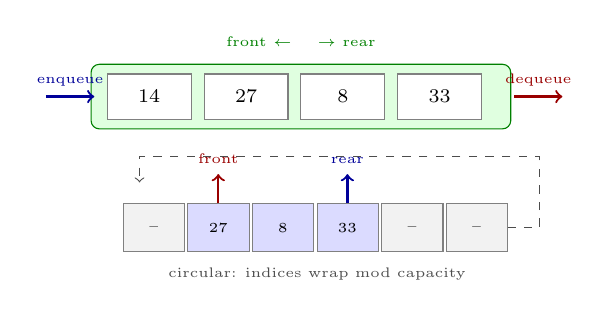
\begin{tikzpicture}[scale=0.82, every node/.style={font=\scriptsize}]
  \draw[fill=green!12, draw=green!50!black, rounded corners=3pt] (0,0) rectangle ++(6.5,1.0);
  \foreach \i/\v in {0/14,1/27,2/8,3/33} {
    \draw[fill=white, draw=black!50] (0.25+\i*1.5,0.15) rectangle ++(1.3,0.7);
    \node at (0.25+\i*1.5+0.65,0.5) {\v};
  }
  \draw[->, thick, blue!60!black] (-0.7,0.5) -- (0.05,0.5) node[midway, above, font=\tiny] {enqueue};
  \draw[->, thick, red!60!black] (6.55,0.5) -- (7.3,0.5) node[midway, above, font=\tiny] {dequeue};
  \node[font=\tiny, green!50!black] at (3.25,1.35) {front $\leftarrow$ \quad $\to$ rear};
  \begin{scope}[yshift=-1.9cm, xshift=0.5cm]
    \foreach \i/\v/\c in {0/--/gray!10,1/27/blue!14,2/8/blue!14,3/33/blue!14,4/--/gray!10,5/--/gray!10} {
      \draw[fill=\c, draw=black!50] (\i*1.0,0) rectangle ++(0.95,0.75);
      \node at (\i*1.0+0.47,0.37) {\tiny \v};
    }
    \draw[->, thick, red!60!black] (1*1.0+0.47,0.75) -- ++(0,0.45) node[above, font=\tiny] {front};
    \draw[->, thick, blue!60!black] (3*1.0+0.47,0.75) -- ++(0,0.45) node[above, font=\tiny] {rear};
    \draw[->, dashed, gray!60!black] (5*1.0+0.95,0.37) -- ++(0.5,0) -- ++(0,1.1) -- ++(-6.2,0) -- ++(0,-0.4);
    \node[font=\tiny, gray!60!black] at (3.0,-0.35) {circular: indices wrap mod capacity};
  \end{scope}
\end{tikzpicture}
\caption{Queue (FIFO) and circular-buffer array implementation with \texttt{front}/\texttt{rear} wrapping.}
\label{fig:queue}
\end{figure}

Circular buffer: store \texttt{front}, \texttt{size}, \texttt{cap}; $\texttt{rear}=(\texttt{front}+\texttt{size})\bmod\texttt{cap}$. Enqueue/dequeue adjust pointers modulo \texttt{cap}; no shifting.

% ============================================================
\section{Deques}
\label{sec:deques}
A \emph{deque} (double-ended queue) allows push/pop at \emph{both} ends in $\Theta(1)$. Implemented by doubly linked list or a circular buffer with two pointers. C++ \texttt{deque} gives $O(1)$ random access plus $O(1)$ ends.

\begin{figure}[h]
\centering
\begin{tikzpicture}[scale=0.82, every node/.style={font=\scriptsize}]
  \draw[fill=violet!10, draw=violet!50!black, rounded corners=3pt] (0,0) rectangle ++(7.0,1.0);
  \foreach \i/\v in {0/14,1/27,2/8} {
    \draw[fill=white, draw=black!50] (0.5+\i*1.4,0.15) rectangle ++(1.2,0.7);
    \node at (0.5+\i*1.4+0.6,0.5) {\v};
  }
  \draw[{Stealth}-{Stealth}, thick, violet!70!black] (-0.6,0.5) -- (0.3,0.5);
  \draw[{Stealth}-{Stealth}, thick, violet!70!black] (4.9,0.5) -- (7.6,0.5);
  \node[font=\tiny, violet!70!black] at (3.0,1.35) {push/pop at either end $O(1)$};
  \node[font=\tiny, gray!60!black] at (3.5,-0.35) {deque generalises both stack and queue};
\end{tikzpicture}
\caption{Deque supports operations at both ends, subsuming stack and queue.}
\label{fig:deque}
\end{figure}

\begin{lstlisting}[language=Python]
from collections import deque
dq = deque([27, 8])
dq.appendleft(14)   # O(1) left push
dq.append(33)       # O(1) right push
dq.popleft()        # O(1) -> 14
dq.pop()            # O(1) -> 33
\end{lstlisting}

Use cases: sliding-window maximum (monotone deque, Ch.~8), work stealing, palindrome checking, undo/redo with two stacks.

% ============================================================
\section{Implementations Compared}

\begin{table}[h]
\centering
\small
\begin{tabular}{lccc}
\toprule
Structure & Array & Linked list & Circular buf. \\
\midrule
Stack push/pop & $O(1)$ & $O(1)$ & --- \\
Queue enq/deq & $O(n)$ shift & $O(1)$ & $O(1)$ \\
Deque both ends & $O(n)$ & $O(1)$ & $O(1)$ \\
Cache locality & excellent & poor & excellent \\
\bottomrule
\end{tabular}
\caption{Implementation trade-offs. Circular buffer wins for queue/deque on arrays.}
\label{tab:stack-queue-impl}
\end{table}

% ============================================================

% --- Additional: Applications deep dive ---
\section{Applications: Matching, Evaluation, BFS Preview}
\label{sec:applications-sq}
\textbf{Postfix evaluation.} Scan tokens left to right: push operands; on operator pop two, apply, push result. Example $3\,4\,+\,2\,\times = 14$. Infix $\to$ postfix via shunting-yard (operator stack) handles precedence.

\textbf{Function calls.} The call stack stores frames (locals, return address). Recursion depth $=$ stack height; tail recursion can be optimised to iteration.

\textbf{BFS preview.} A queue gives level-order traversal (Ch.~3) and shortest paths in unweighted graphs (Ch.~7). Replacing the queue with a stack yields DFS --- same code, different data structure, radically different order.

\begin{lstlisting}[language=Python]
# Postfix evaluator -- O(n)
def eval_postfix(tokens):
    st = []
    for tok in tokens:
        if tok in "+-*/":
            b, a = st.pop(), st.pop()
            st.append(str(eval(f"{a}{tok}{b}")))
        else:
            st.append(tok)
    return int(st[0])
# eval_postfix(["3","4","+","2","*"]) == 14
\end{lstlisting}

\begin{remark}
Monotone deque for sliding-window maximum: maintain decreasing deque of candidates; each element enters and leaves once --- $O(n)$ for window size $k$ over $n$ elements, previewing Ch.~8.
\end{remark}

\section{Chapter Notes}
CLRS Ch.~10.1, Weiss Ch.~3.3--3.6. STL: \texttt{stack} and \texttt{queue} are adapters over \texttt{deque} by default; \texttt{priority\_queue} is in Ch.~5.

% ============================================================
\section{Exercises}
\label{sec:ch02-exercises}
\begin{enumerate}[label=E2.\arabic*, leftmargin=*, itemsep=0.7em]
    \item \textbf{Circular queue.} Implement queue with array \texttt{A[0..cap-1]}, integers \texttt{front}, \texttt{sz}. Give \texttt{enqueue}, \texttt{dequeue}, \texttt{isEmpty}, \texttt{isFull} in $O(1)$. How do you distinguish full vs.\ empty?
    \item \textbf{Two stacks, one array.} Use a single array of size $n$ for two stacks growing from opposite ends. Give push/pop for each and prove overflow iff total items $>n$.
    \item \textbf{Postfix evaluation.} Evaluate $5\,1\,2\,+\,4\,*\;+\,3\,-$ with a stack, showing contents after each token. Write $O(n)$ algorithm for general postfix over $+,-,\times,/ $.
    \item \textbf{Queue via stacks.} Implement queue using two stacks with amortised $O(1)$ enqueue/dequeue. Prove amortised bound via potential $\Phi=$ size of input stack.
    \item \textbf{Deque min.} Design deque supporting \texttt{pushFront/Back}, \texttt{popFront/Back}, and \texttt{getMin} in $O(1)$ amortised (hint: auxiliary monotone deque).
\end{enumerate}
% End of Chapter 2
